\chapter{Background and Problem Definition}
\label{chap:backgroud}
\adjustmtc
\minitoc

Our contributions bridge standard \ai paradigms and developmental psychology to investigate two fundamental research questions  (1) the language acquisition problem (self-organisation of cultural conventions) and (2) the open-ended skill acquisition problem (self-organisation of trajectories). In this chapter, we will first present standard \ai problems and their associated families of algorithmic solutions before getting into the specifications of the two problems we investigate.

\section{Background: Standard \ai Paradigms}



\subsection{Reinforcement Learning}

\paragraph{Problem}

In a Reinforcement Learning problem, an agent learns to perform sequences of actions in an environment by maximizing some notion of cumulative reward~\citep{sutton2018reinforcement}.  The agent interacts with the environment in the form of a temporal sequence unfolding from time $t=0$ to time $t=T$, $T$ being the episode horizon and representing the lifetime of the agent (potentially variable or infinite). \rl problems are commonly framed as Markov Decision Processes (\mdps):
\begin{equation}
	\m{M}\,=\,\{\m{S},\,\m{A},\,\m{T},\,\rho_0,\,R\}	
\end{equation}
where $\m{S}$ and $\m{A}$ are respectively the state and action spaces, $\m{T}$ is the transition function that dictates how actions impact the world (lead to the next state), $\rho_0$ is the initial state distribution and $R$ is the reward function. 
%\textbf{Interactions. }  
At the beginning of an episode, the agent starts in the initial state $s_0 \sim \rho_0(\mathcal{S})$. At each time step the agents takes action $a_t \in \mathcal{A}$ and observes the next state $s'=s_{t+1} \in \m{S}$ and the reward $r_{t+1}=R(s_t,a_t)$. A diagram of interaction is given in figure~\ref{fig:rl_interacvtions}.
\begin{figure}[!h]
\centering
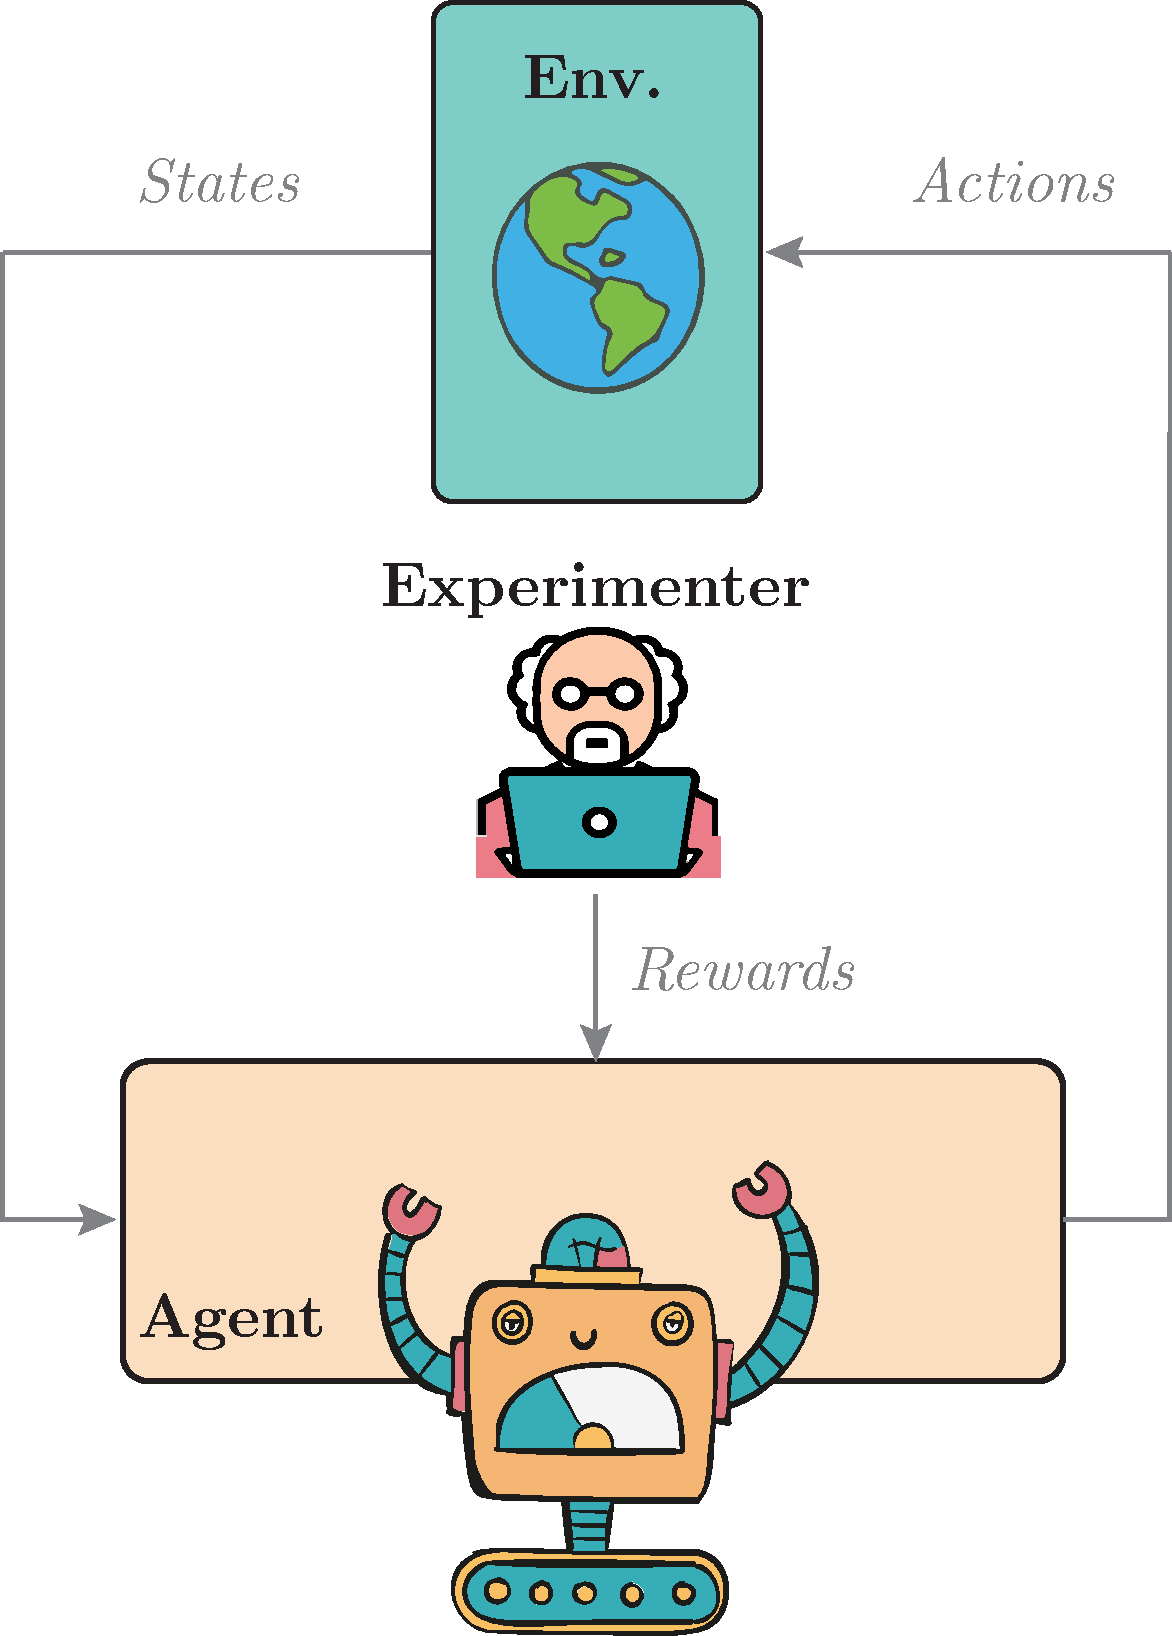
\includegraphics[width=0.3\textwidth]{background/rl_interactions.pdf}	
\caption{Interactions in a \rl loop}
\label{fig:rl_interacvtions}
\end{figure}
The transition function $\m{T}$ gives the distribution of the following states from the current state and action: $\m{T}=P_E(.|s, a)$ with $P_E$ being the (potentially stochastic) dynamics of the environment. In an \mdp, the transition function must respect the \textit{Markov property}: a future state ($s'$) must only depend on the current state ($s$) and not on its predecessor, i.e. the transition function is memoryless. 
\begin{equation}
 P_E(s_{t+1}|s_t,a_t) = P_E(s_{t+1}|s_0,\dots,s_t,a_t)	
\end{equation}

In a \rl problem, the behavior of the agent is expressed as a \textit{policy} $\pi : \m{S} \rightarrow \m{A}$ that predicts the next action $a$ based on the current state $s$. This policy can be stochastic ${a_t\sim\pi(.|s_t)}$ or deterministic $a_t=\bar{\pi}(s_t)$. When agents interact in an environment, they produce \textit{trajectories}. A trajectory is a sequence of states and actions $\tau=(s_0,a_0,\dots,s_T,a_T)$. When both the dynamics of the environment and the policy of the agent is stochastic, the probability of a trajectory is:
\begin{equation}
P(\tau|\pi)=\rho_0(s_0)\prod_{t=0}^{T-1} P_E(s_{t+1}|s_t,a_t)\pi(a_t|s_t)	
\label{eq:traj_dist}
\end{equation}
The objective of the agent is to maximize the cumulative reward computed over trajectories ($R^{tot}$). When computing the aggregation of rewards,  we often introduce discounting and give smaller weights to delayed rewards. The return of a trajectory is therefore:
\begin{equation}
R^{tot}(\tau) = \sum_{t=0}^{T} \gamma^{t}R(s_t,a_t)
\end{equation}
with $\gamma \in ]0,1]$ being a constant discount factor. We call the optimal policy $\pi^*$, the behavior that maximizes the expected return:
\begin{equation}
	\pi^*=\argmax_\pi \expect{\tau\sim\pi}[R^{tot}(\tau)] = \argmax_\pi \expect{(a_t\sim\pi, s_t\sim P_E)}\left[\sum_{t=0}^{T} \gamma^{t}R(s_t,a_t)\right]
\end{equation}
The reward function plays therefore a crucial role in a \rl problem as its maximization will directly shape the behavior of the agent.

\paragraph{Value Functions}

Most \rl algorithms rely on the definition of \textit{value} and \textit{action-value} functions:
\begin{itemize}[noitemsep]
	 \item The value function $V_\pi(s)$ of a policy $\pi$ gives the expected return of a trajectory starting from $s$ and following $\pi$. 
	 \item The action-value function $Q_\pi(s,a)$ is the expected return of the trajectory taking action $a$ from state $s$ before following $\pi$ from the next state $s'$. 
\end{itemize}
Action-value functions are powerful because they allow us to instantly assess the quality of a situation without waiting for the end of the trajectory. The value and action-value function obey the Bellman expectation equations~\citep{sutton1998intra}, a recursive definition that states that the value of a certain state (when following policy $\pi$) is equal to the sum of the instantaneous reward and the value from the next state.
\begin{equation}
\left\{
\begin{split}
	V_\pi(s) & = \underset{(a\sim\pi, s'\sim P_E)}{\mathbb{E}}\left[R(s,a) + \gamma V_\pi(s')\right]  \\
	Q_\pi(s,a) &= \underset{s'\sim P_E}{\mathbb{E}}\left[ R(s,a) + \gamma \underset{a' \sim \pi}{\mathbb{E}}[Q_\pi(s',a')]\right]
\end{split}
\right.	
\end{equation}
The value and action-value functions also follow the Bellman optimality equation where expectations over actions are replaced by max operators.
\begin{equation}
\left\{
\begin{split}
	V^*(s) & = \max_a\underset{s'\sim P_E}{\mathbb{E}}\left[R(s,a) + \gamma V^*(s')\right]  \\
	Q^*(s,a) &= \underset{s'\sim P_E}{\mathbb{E}}\left[ R(s,a) + \gamma \max_{a'}[Q^*(s',a')]\right]
\end{split}
\right.	
\end{equation}
Acting greedily with respect to the optimal action-value function gives the optimal policy:
\begin{equation}
\pi^*(s) = \argmax_a Q^*(s,a)	
\end{equation}


Computing $Q^*$ is therefore a way to solve a \rl problem. When agents have access to perfect knowledge of the dynamic of the environment ($P_E$) and when the dimensionality of $\m{S}$ and $\m{A}$ is small, they can do planning to find the optimal action-value function via Dynamic Programming~\citep{bellman1966dynamic} for instance. Planning approaches that leverage the transition function of the environments are called \textit{model-based} \rl algorithms. They are opposed to \textit{model-free} \rl algorithms that do not use $P_E$ but interact directly with a simulator (with transition function $P_S$).

Because the present research builds on both families of solutions, we detail the techniques used for each in the following paragraphs. We first briefly detail the \textit{Monte-Carlo Tree Search} planning algorithm (\mcts)~\citep{browne2012mcts} used in our first experimental contribution (in chapter~\ref{chap:abig}) and then introduce the deep \rl algorithms used in chapter~\ref{chap:imagine}.

\paragraph{Model-based \rl with \mcts:}

\mcts is a tree-search algorithm that seeks to identify the optimal policy by finding the action with the highest Q-value. To this end, \mcts build an estimate $\hat{Q}(s,a)$ for $a \in \m{A}$ in a given state $s$ and acts greedily with respect to this estimate. Each node of the tree is a state $s$ while edges are the potential actions. The \mcts algorithm grows the tree iteratively using an exploration/exploitation tradeoff to efficiently refine $\hat{Q}$ in promising regions of the \mdp. More specifically, each iteration of the \mcts algorithm contains four steps:
\begin{enumerate}[noitemsep]
	\item \textbf{Selection:} In the selection phase, the \mcts algorithm starts from the root node and uses a tree policy to decide which node to expand. The tree policy is guided by an evaluation function ($UCT$) and stops when a node with remaining actions to explore is reached. 
	\item \textbf{Expansion:} Once a leaf node is reached, a new action $a$ is sampled among the non-explored ones and the corresponding node is computed using the transition function $s' \sim P_E(.|s,a)$
	\item \textbf{Simulation:} From the newly created node corresponding to state $s'$, a simulation policy $\pi_{sim}$ is used to draw a full trajectory (until termination or for a predefined horizon) and compute return $R^{tot}$. $\pi_{sim}$ is often a random policy.
	\item \textbf{Backpropagation:} $R^{tot}$ is backpropagated to the root node as indicated in figure~\ref{fig:mcts_steps}.
\end{enumerate}
For the tree policy evaluation function, we use the Upper Confidence Bound~\citep{auer_finite-time_2002}: $UCT = \frac{1}{k}\sum_{i=0}^{k} R^{tot}_{i} + C\sqrt{\frac{\text{ln}(n)}{k}}$ where $k$ is the number of completed trajectory going through node $s$ and $n$ is the number of iterations. The first term of $UCT$ is an estimation of the expected return while the second term encourages the tree policy to explore unexpanded nodes.
\begin{figure}[!h]
\centering
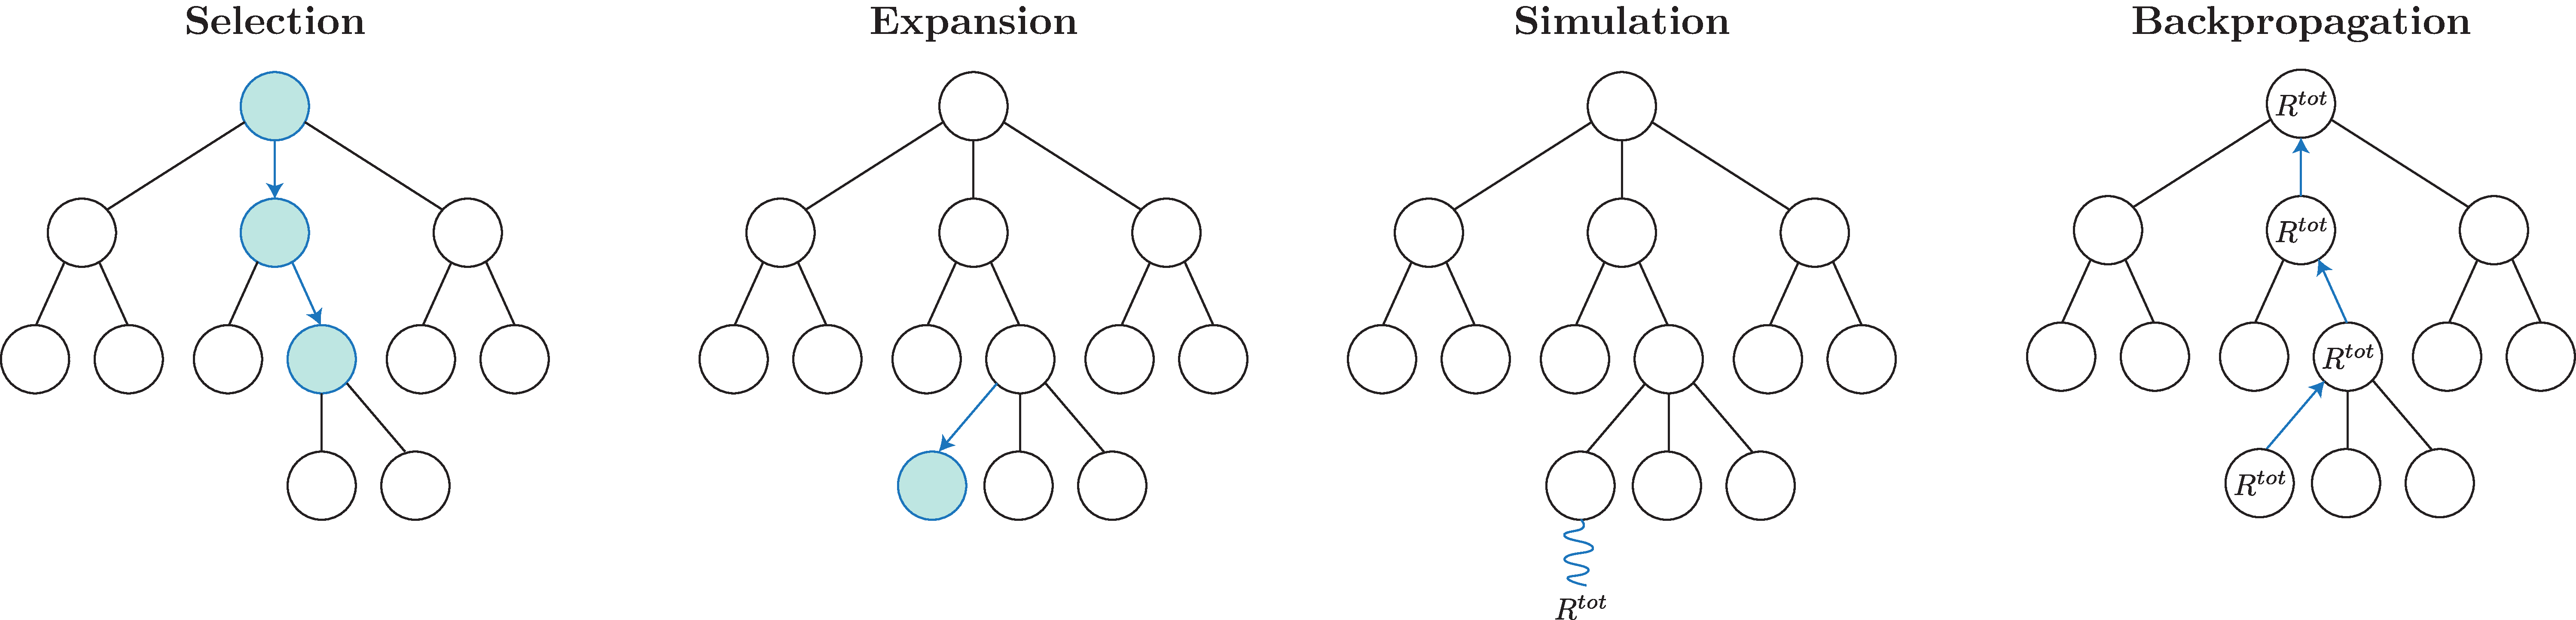
\includegraphics[width=1\textwidth]{background/mcts_4_steps.pdf}
\caption{The four steps of an \mcts iteration}
\label{fig:mcts_steps}	
\end{figure}

\paragraph{Model-free \rl with Q-learning:}

Some of the experimental contributions of this research build on the \textit{Deep Deterministic Policy Gradient} (\ddpg) algorithm~\citep{lillicrap2015continuous}. \ddpg derives from \textit{Deep Q-Networks} (\dqn) \citep{mnih2015human} which is itself a deep learning implementation of the standard \textit{Q-learning} algorithm~\citep{watkins_q-learning_1992}.  In this paragraph, we propose to detail the steps that allow building DDPG from Q-learning. 

\textbf{Q-learning} is an \textit{off-policy} \rl algorithm. Off-policy algorithms, in contrast to on-policy algorithms, learn to approximate the action-value $Q^*$ of an optimal policy independently of the policy used for data collection. Q-learning relies on transitions $(s,a,r,s')$ collected by a policy $\pi_c$ interacting with a simulator $P_S$. Assuming that $Q$ is a linear combination of features ($\phi$): $Q(s,a;\theta)=\theta^T\phi(s,a)$, the algorithm iteratively learns to approximate $Q^*$ by minimizing the temporal difference error (TD-error):
\begin{equation}
\m{L}_i=\underset{(s\sim P_S, a\sim\pi_c)}{\mathbb{E}} \left[(y_i - Q(s,a;\theta_i))^2 \right] \text{ with } y_i = \underset{s'\sim P_S}{\mathbb{E}}\left[r +\gamma \max_{a'}Q(s',a';\theta_{i-1})\right] 
\label{eq:loss_td}
\end{equation}
In the original formulation of the Q-learning algorithm by \citet{watkins_q-learning_1992}, they consider a tabular setting and store the Q-values at each iteration in a table ($Q_i[s,a]$) instead of using linear function approximations. The update of the table writes:
\begin{equation}
Q_{i+1}[s,a] \leftarrow Q_i[s,a] + \alpha \left(r + \gamma\max_{a'}Q_i[s',a'] - Q_i[s,a]\right)
\end{equation}


\textbf{\dqn} proposes to represent the action-value function with deep neural networks: $Q(s,a;\theta)$ with parameters $\theta$. The architecture of the network takes a state $s$ as input and outputs the value of each action $Q(s,a) \forall a \in \mathcal{A}$. Thus \dqn only works with discrete action space. When differentiating \eq{eq:loss_td} with respect to the neural network parameters, we get:
\begin{equation}
	\nabla_{\theta_i }\m{L}_i(\theta_i ) = \underset{(s\sim P_S, a\sim\pi_c)}{\mathbb{E}} \left[(y_i - Q(s,a;\theta _i))\nabla_{\theta_i }Q(s,a;\theta _i)\right]
\end{equation}
During differentiation, one has to pay particular attention to freezing the weights of the network when evaluating $y_i$. Deep neural networks are known to exhibit training instabilities. In order to stabilize learning, \citet{mnih2015human} proposed two main innovations: 
\begin{itemize}[noitemsep]
\item \textit{Experience Replay}: The agent uses a replay buffer to store transitions during interactions. During learning, the transitions are then sampled uniformly to perform updates. This enables breaking the correlation between successive transitions and reusing them.
\item \textit{Target network}: A target network is used to compute target $y$. This network is initialized with the actual Q-network ($Q_{targ}(s,a;\theta_{targ})=Q(s,a;\theta$) but updated less frequently than the actual Q-network. Updates are often performed using \textit{Polyak averaging}~\citep{polyak1992}: $\theta_{targ} \leftarrow \rho\theta_{targ} + (1-\rho)\theta$ with $\rho$ being the polyak factor.
\end{itemize}

\textbf{\ddpg} is an adaptation of \dqn to continuous action space. The challenge of dealing with continuous actions is to act greedily with respect to the learned Q-value. i.e. to evaluate $\argmax_a Q(s,a)$. To overcome this, \ddpg concurrently learns a deterministic policy with the Q-function. This policy is a parametrized network $\pi(s;\phi)$ with parameters $\phi$ and is obtained by gradient ascent. Moreover, since $\pi(s;\phi) \approx \argmax_a Q(s,a,\theta)$ it can be injected in \eq{eq:loss_td}. We, therefore, have the two following losses to optimize:
\begin{equation}
\left\{
\begin{split}
	\m{L}_{\pi_\phi} &= \underset{(s\sim P_S)}{\mathbb{E}}\left[Q_\theta(s,\pi_\phi(s))\right] \quad \quad \quad \quad \text{ (Policy loss)}\\
	\m{L}_{Q_\theta} &= \underset{(s\sim P_S,a\sim\pi_c)}{\mathbb{E}}\left[(y- Q_\theta(s,a))^2 \right] \quad \text{(Q-value loss)}\\
	& \text{with } y = \underset{s'\sim P_S}{\mathbb{E}}\left[r +\gamma Q_\theta(s',\pi_\phi)\right]
\end{split}
\right.
\end{equation}
where parameter dependencies have been subscripted.

\paragraph{Other model-free \rl algorithms}

There are numerous algorithms within the field of \drl, including on-policy methos like \textsc{trpo}~\citep{pmlr-v37-schulman15}, \textsc{ppo}~\citep{ppo2017} as well as more advanced off-policy approaches like \textsc{td3}~\citep{pmlr-v80-fujimoto18a} and \textsc{sac}~\citep{pmlr-v80-haarnoja18b}.


\subsection{Imitation Learning}

\paragraph{Problem}

\textit{Imitation Learning} (\il)~\citep{pommerleau1988BC,schaal1996learning,osa2018algorithmic} is a field that considers an agent learning in a \mdp in which the reward function is not explicitly defined, but where the agent can observe demonstrations of the task it is intended to perform. \il is particularly useful in situations where it is difficult for the experimenter to design a task-specific reward function, but demonstrations are available. A classic example from the literature is the application of \il to self-driving cars. It is impractical to specify a reward function for the task of driving as successful drivers constantly adjust their criteria to adapt to the various events that occur on the road. However, there is a vast amount of video footage of people driving that could potentially be utilized by the agent to learn.

\begin{figure}[!h]
\centering
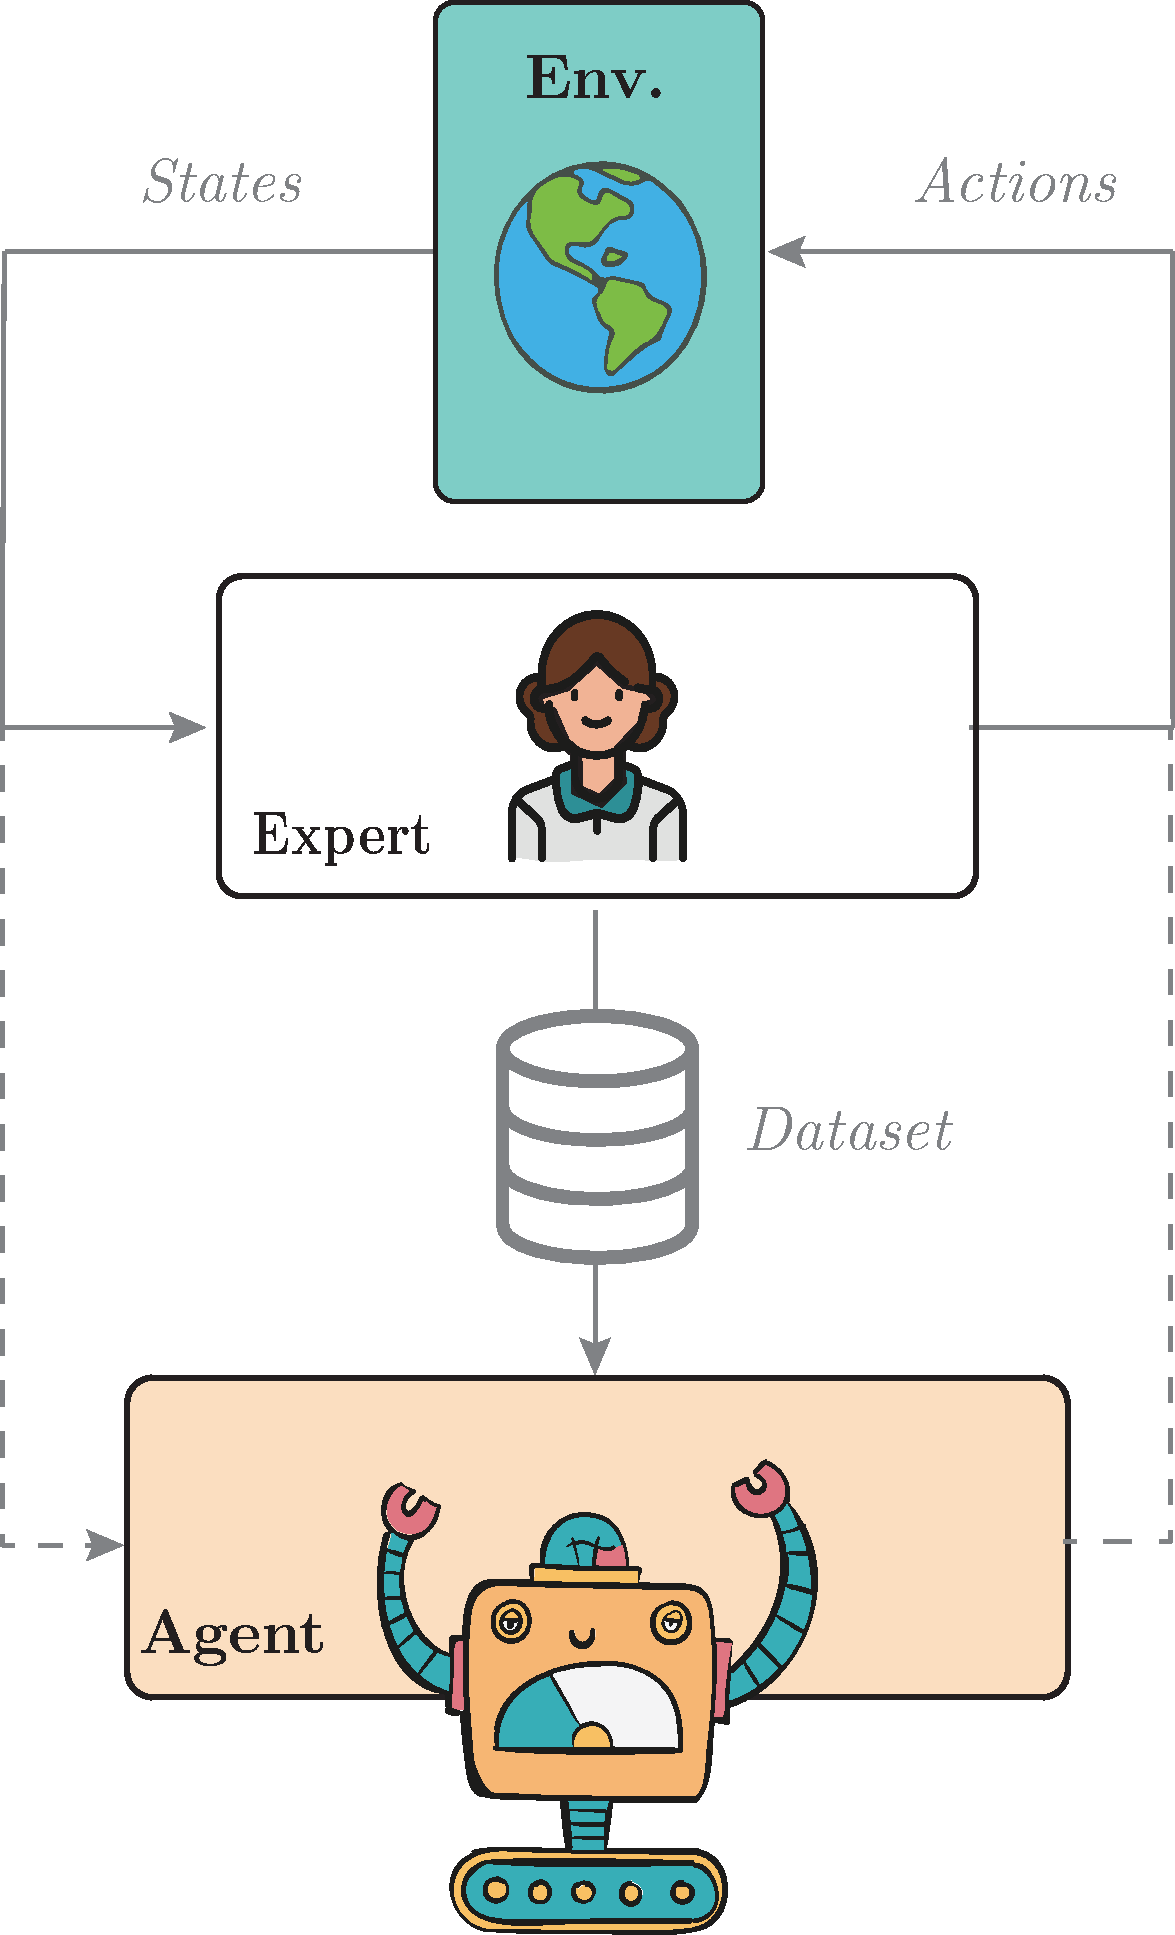
\includegraphics[width=0.3\textwidth]{background/il_interactions.pdf}	
\caption{Interactions in a \il problem. The agent never interacts with the environment during learning but can interact with it to test its behavior (dashed lines).}
\label{fig:il_interacvtions}
\end{figure}

A standard way of formalizing the \il problem is to find a policy that minimizes the divergence between the expert and learner data distribution. Provided a dataset $\m{D}=\{(\tau_i)\}_{i=1}^N$ containing expert trajectories of features $\tau = [\phi_0,\dots, \phi_T]$. If $q_{\pi^*}(\phi)$ is the distribution of features induced by the expert's policy (supposed optimal $\pi^*$) and $p_\pi(\phi)$ is the distribution of features induced by the learners' policy ($\pi$), the goal of \il is to find policy $\hat{\pi}$ such that:
\begin{equation}
\hat{\pi} = \argmin_{\pi}D(q_{\pi^*}(\phi),p_\pi(\phi))
\end{equation}
with $D$ being a measure of differences between probability distributions such as the well-known Kullback-Leibler (KL) divergence.

\paragraph{Behavioral Cloning}

An intuitive way of solving an \il problem is to frame it as a supervised learning setting and do \textit{Behavioral Cloning}(\bc). Given a dataset of trajectories $\m{D}=\{(\tau_i)\}_{i=1}^N$ with  $\tau=[(s_0,a_0) \dots (s_T,a_T)]$, one directly minimizes the cross entropy loss:
\begin{equation}
\m{L}_\pi = -\expect{(s,a)~\sim\m{D}}[\log\pi(s,a)]
\end{equation}
Minimizing this cross-entropy loss is in fact equivalent to minimizing the KL-divergence between the trajectory distribution of the expert $P(\tau|\pi^*)$ and the trajectory distribution of the learner $P(\tau|\pi)$~\citep{ke2020imitation}:
\begin{equation}
D_{KL}(P(\tau|\pi^*),P(\tau|\pi)) = \underset{\tau \in \m{D}}{\sum}P(\tau|\pi^*)\log\left(\frac{P(\tau|\pi^*)}{P(\tau|\pi)}\right)
\end{equation}
%
Injecting the definition of the trajectory distribution of \eq{eq:traj_dist} we get that:
%
\begin{align}
D_{KL}(P(\tau|\pi^*),P(\tau|\pi)) &= \underset{\tau \in \m{D}}{\sum}P(\tau|\pi^*)\log\left(\prod_{t=0}^{T-1}\frac{\pi^*(a_t|s_t)}{\pi(a_t|s_t)}\right) \\
&= \underset{\tau \in \m{D}}{\sum}P(\tau|\pi^*)\sum_{t=0}^{T-1}\left(\log\pi^*(a_t|s_t) - \log\pi(a_t|s_t)\right) \\
&= \expect{(s,a)\sim\m{D}}\left[\log\pi^*(a_t|s_t) - \log\pi(a_t|s_t)\right]
\end{align}
%
We will use behavioral cloning in chapter~\ref{chap:abig}. \bc is a straightforward method for reproducing expert behavior. However, simple \bc only works if the agent operates in the same region of the state space as the states provided in $\m{D}$. Otherwise, the policy of the learner will progressively deviate from this region accumulating errors at each time step. This compounding error is called \textit{distributional mismatch}. One way of addressing it is to iteratively collect new expert data when needed (in the initially uncovered region of the state space)~\citep{dagger2011}. 

Another limitation of \bc is that it is only able to derive an optimal policy from optimal expert trajectories, meaning that the learned policy will not exceed the performance of the expert. In some applications collecting optimal trajectories is not always possible. As a result, some researchers have turned to \textit{Inverse Reinforcement Learning} (\irl) as an alternative approach.

\paragraph{Inverse Reinforcement Learning}

Similar to \rl, \irl can be understood both as a problem and a category of techniques. The \irl problem consists in recovering the reward function of an expert given a dataset of its trajectories~\citep{ng2000irl}. As such \irl algorithmic solutions followed by \rl can form a solution to the \il problem. The combination of \irl followed by \rl is called \textit{Apprenticeship Learning}~\citep{abbeel2004apprenticeship}. As formalized by \citet{klein2011apprenticeship}, we distinguish mainly three categories of apprenticeship algorithms:
\begin{enumerate}[noitemsep]
\item Feature-expectation-based methods as proposed by \citet{ziebart2008maxentirl} which learn a reward function such that the feature expectation of the optimal policy (according to the learned reward function) is similar to the feature expectation of the expert policy. 
\item Margin-maximization-based methods~\citep{ratlif2006maxmargin}, which formulate IRL as a constrained optimization problem in which the expert's examples have a higher expected cumulative reward than all other policies by a certain margin.
\item Approaches based on the parameterization of the policy by the reward~\citep{neu2007apprenticeship}: If it is assumed that the expert follows a Gibbs policy (or the optimal value function related to the optimized reward function), it is possible to estimate the likelihood of a set of state-action pairs provided by the expert.
\end{enumerate}
%
Recent feature-expectation-based approaches use technics similar to generative adversarial networks (\gan)~\citep{goodfellow2014generative} to imitate complex behavior in high-dimensional environments~\citep{ho2016gail}. Other approaches use ranking of trajectories to reach better-than-demonstrator performances~\citep{brown2020better}. As we do not leverage \irl in our contributions we will not detail these methods (see \citet{arora_survey_2021} for a thorough survey of \irl algorithms).


\subsection{Muli-Goal Reinforcement Learning}



\paragraph{Problem}

By replacing the unique reward function $R$ by the space of reward functions $\m{R}_\m{G}$, \rl problems can be extended to handle multiple goals: $\m{M}\,=\,\{\m{S},\,\m{A},\,\m{T},\,\rho_0,\,\m{R}_\m{G}\}$. The term \textit{goal} should not be mistaken for the term \textit{task}, which refers to a particular \mdp instance. As a result, \textit{multi-task} \rl refers to \rl algorithms that tackle a set of \mdps that can differ by any of their components (\eg $\m{T}$,\,$R$,\,$\m{S}_0$, etc.). The \textit{multi-goal} \rl problem can thus be seen as the particular case of the multi-task \rl problem where \mdps differ by their reward functions. In the standard multi-goal \rl problem, the set of goals\,---\,and thus the set of reward functions\,---\,is pre-defined by engineers. The experimenter sets goals to the agent, and provides the associated reward functions. 


\paragraph{Interactions}

\begin{figure}[!h]
\centering
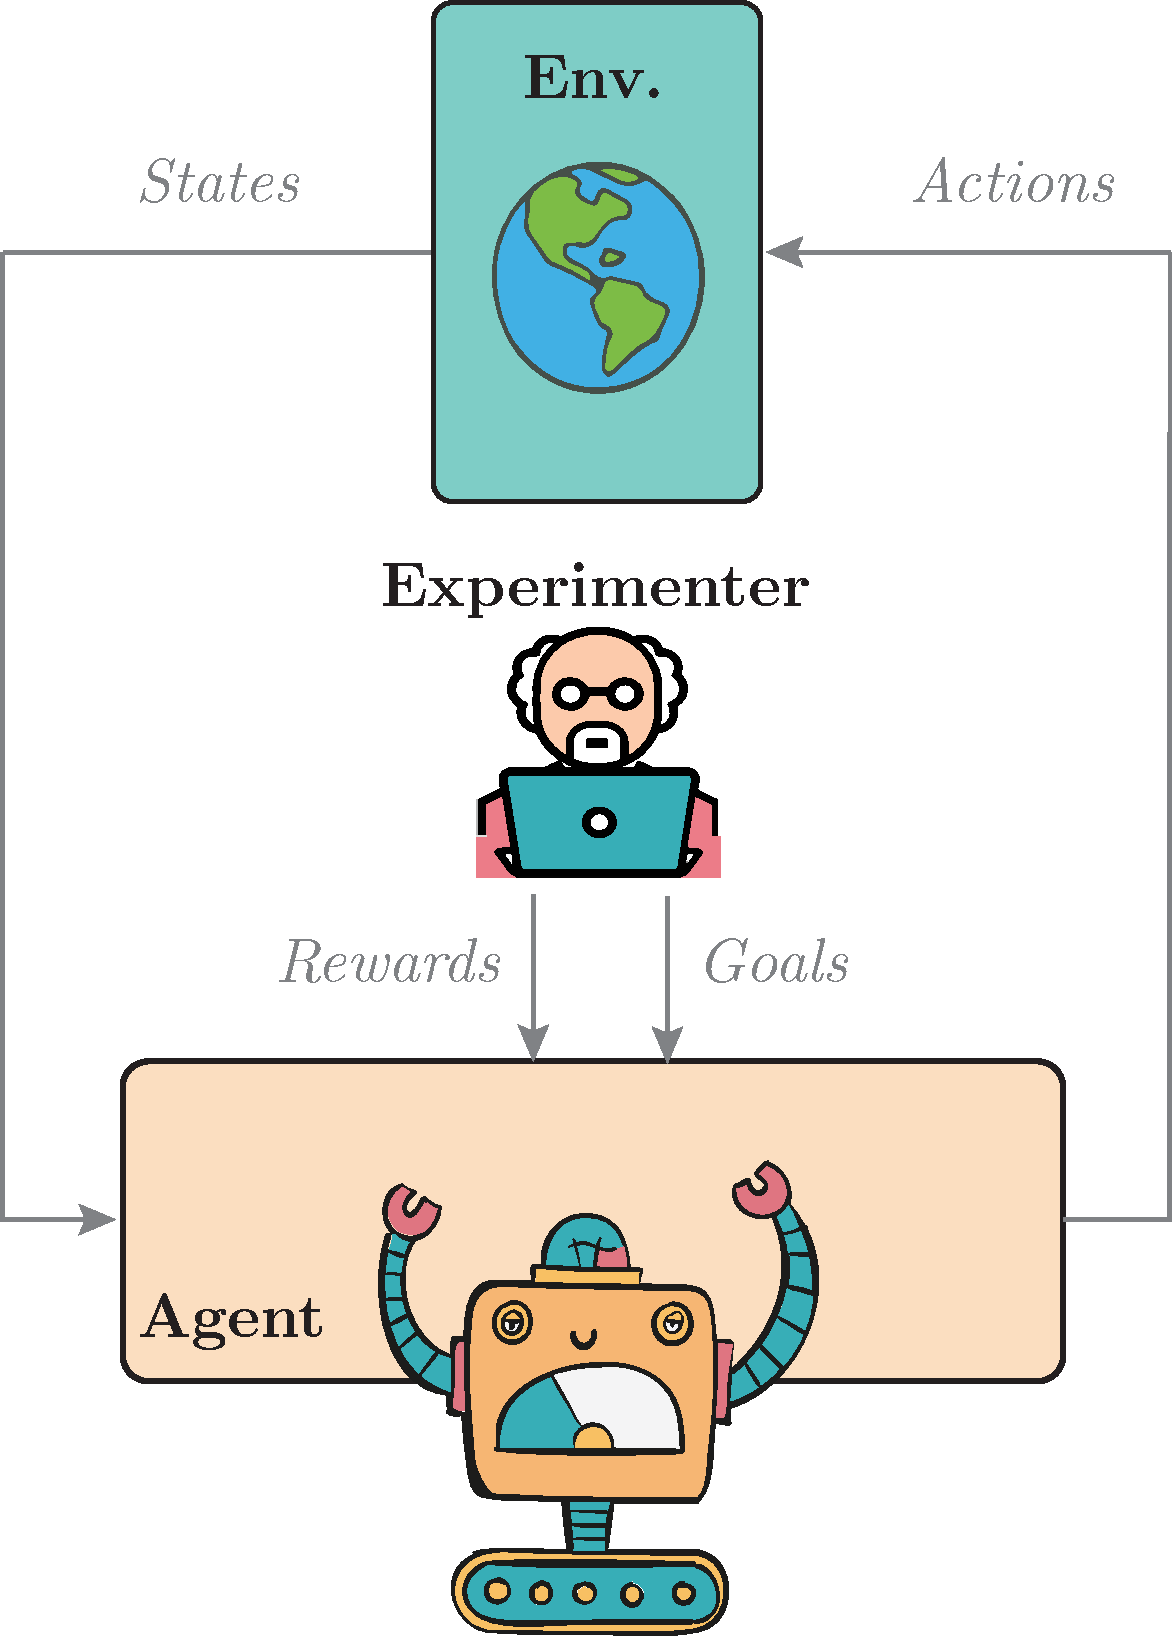
\includegraphics[width=0.3\textwidth]{background/multi_goal_rl_interactions.pdf}	
\caption{}
\label{fig:mg_rl_interacvtions}
\end{figure}


\paragraph{Solution}

Goal-conditioned agents see their behavior affected by the goal they pursue. This is formalized via goal-conditioned policies, that is policies that produce actions based on the environment state and the agent's current goal: $\Pi:\m{S}\times\m{Z}_\m{G}\to\m{A}$, where $\m{Z}_\m{G}$ is the space of goal embeddings corresponding to the goal space $\m{G}$ \cite{schaul2015universal}. Note that ensembles of policies can also be formalized this way, via a meta-policy $\Pi$ that retrieves the particular policy from a one-hot goal embedding $z_g$ \cite{kaelbling1993learning,sutton2011horde}.

The idea of using a unique \rl agent to target multiple goals dates back to \cite{kaelbling1993learning}. Later, the \horde architecture proposed to use interaction experience to update one value function per goal, effectively transferring to all goals the knowledge acquired while aiming at a particular one \cite{sutton2011horde}. In these approaches, one policy is trained for each of the goals and the data collected by one can be used to train others.

Building on these early results, \cite{schaul2015universal} introduced \textit{Universal Value Function Approximators} (\uvfa). They proposed to learn a unique goal-conditioned value function and goal-conditioned policy to replace the set of value functions learned in \horde. Using neural networks as function approximators, they showed that \uvfas enable transfer between goals and demonstrate strong generalization to new goals.

The idea of \textit{hindsight learning} further improves knowledge transfer between goals \cite{kaelbling1993learning,andrychowicz2017hindsight}. Learning by hindsight, agents can reinterpret a past trajectory collected while pursuing a given goal in the light of a new goal. By asking themselves, \textit{what is the goal for which this trajectory is optimal?}, they can use the originally failed trajectory as an informative trajectory to learn about another goal, thus making the most out of every trajectory \cite{eysenbach2020rewriting}. This ability dramatically increases the sample efficiency of goal-conditioned algorithms and is arguably an important driver of the recent interest in goal-conditioned \rl approaches.


\subsection{Multi-Agent Reinforcement Learning}

\paragraph{Problem}

\todo{markov games}

\paragraph{Interactions}

\begin{figure}[!h]
\centering
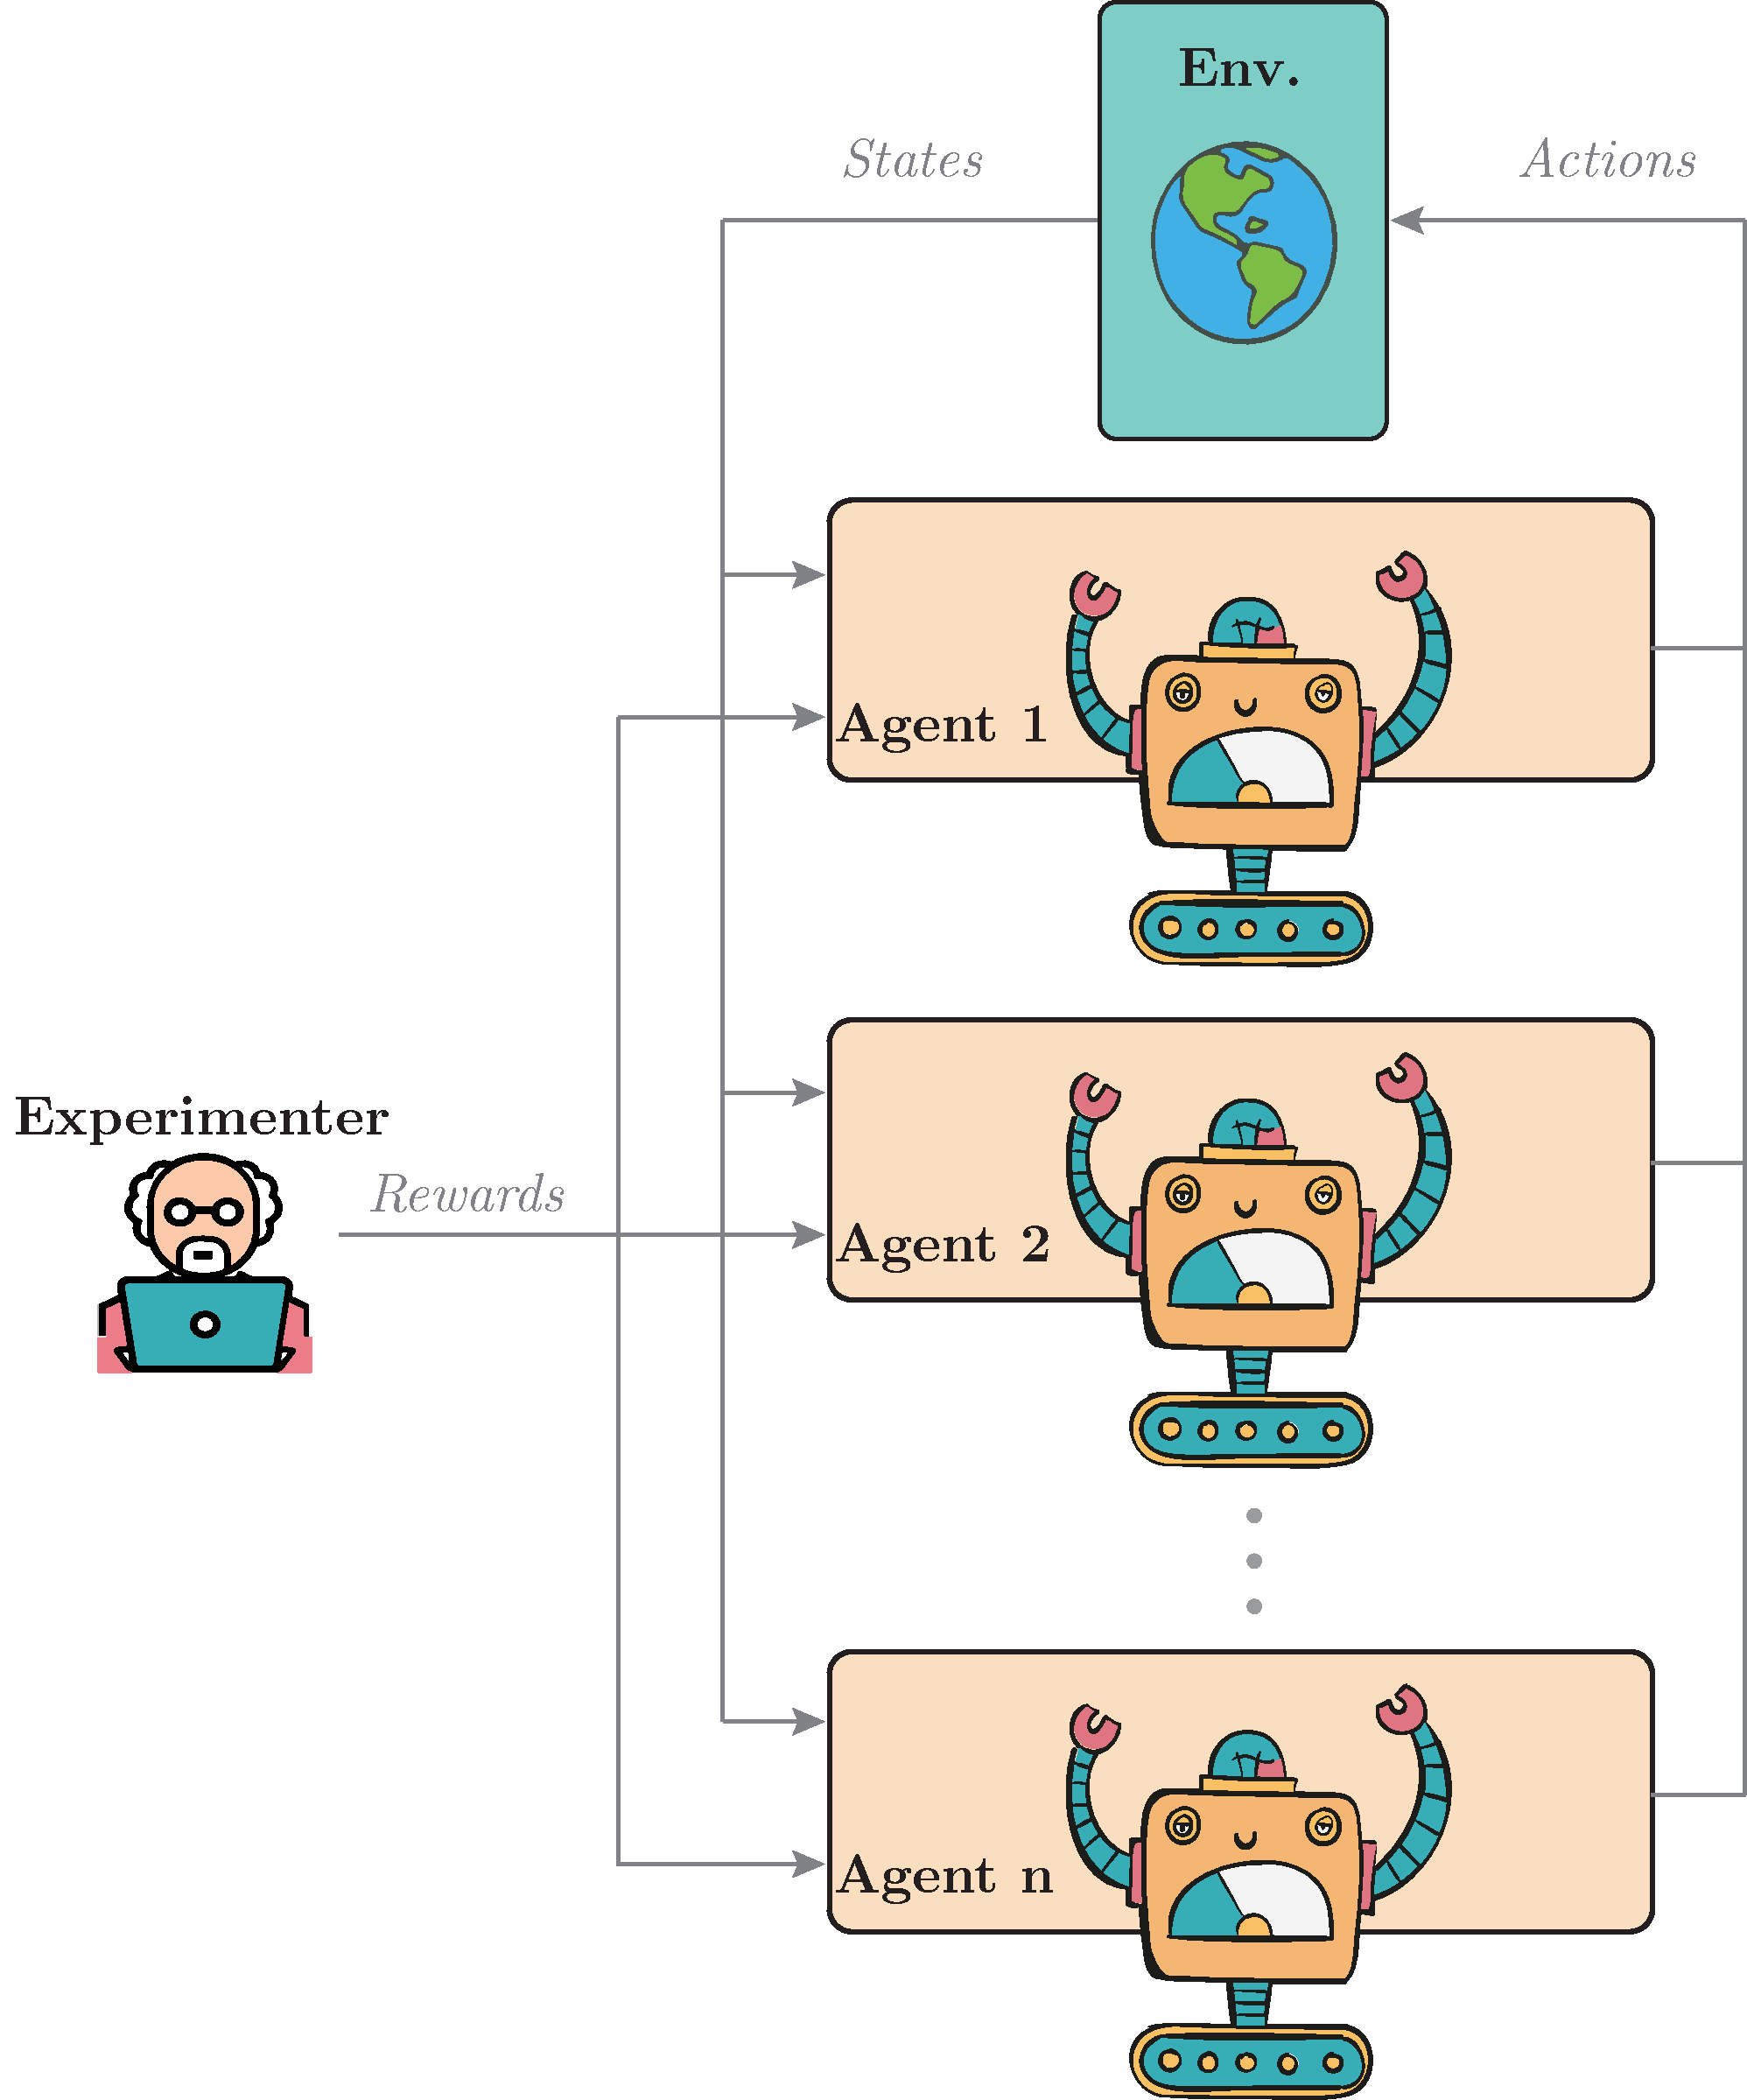
\includegraphics[width=0.5\textwidth]{background/marl_interactions.pdf}	
\caption{}
\label{fig:marl_interacvtions}
\end{figure}


\paragraph{Solution}

\todo{maddpg centralized trainign decentralized execution}

\section{Problem Definition: Developmental AI}

\todo{objective is very different from engineering problems in standard ai paradigms. we don't have clear and rigurous problem definition, we rather analyze all the facets of emerging phenomenon.}

\gls{Self-organization} is a process by which spontaneously ordered patterns and structures emerge in a system without the need for central control or external guidance. It is a bottom-up process, meaning that it arises from the interactions and behaviors of the individual components within the system, rather than being imposed on the system from the top down. Self-organization can occur in various systems, including biological, chemical, physical, and social systems. It is often characterized by the emergence of complex, dynamic patterns and structures that exhibit behaviors that are not present in the individual components alone.



\todo{add definition of self-organization} \citet{oudeyer2005selforganization} \citet{steels1997evolution}

\todo{example}

\subsection{Language Acquisition Problem}


\paragraph{Language Games}

\paragraph{Neural Network Communicating Agents}

\paragraph{MARL communication}

\paragraph{How to evaluate self-organizing communicating agents?}


\subsection{Open-ended Skill Acquisition Problem}

\paragraph{autotelic}

\paragraph{How to evaluate autotelic agents?}



